\documentclass[12pt,a4paper]{report}

%adjust your page margins here
\usepackage[top=0.70in, bottom=0.70in, left=0.8in,right=0.80in]{geometry} % setting the page alignment with this package
\usepackage[pdftex]{graphicx} %for embedding images
\usepackage[%dvips, % commented for pdflatex
bookmarks,  colorlinks=false]{hyperref} %for creating links in the pdf version and other additional pdf attributes, no effect on the printed document
\hypersetup{%
    pdfborder = {0 0 0}
}
\usepackage[final]{pdfpages} %for embedding another pdf, remove if not required
\usepackage{float} %used for figure placement with H as a parameter
\usepackage{hyperref}
\usepackage{pslatex} % for times new roman, old package, but works
\usepackage{array} % for making text bold in table
\usepackage{setspace}
\usepackage{float}
\usepackage{enumerate}
\usepackage{longtable}
\usepackage{graphicx}
\usepackage{caption}
\usepackage[list=true,listformat=simple]{subcaption}

\usepackage[font=small,labelfont=bf]{caption}
\def\figurename{\textbf{Figure }}

\usepackage{listings}
\usepackage{color}

\definecolor{dkgreen}{rgb}{0,0.6,0}
\definecolor{gray}{rgb}{0.5,0.5,0.5}
\definecolor{mauve}{rgb}{0.58,0,0.82}
 
\lstset{ %
  language=Java,                % the language of the code
  basicstyle=\footnotesize,           % the size of the fonts that are used for the code
  numbers=left,                   % where to put the line-numbers
  numberstyle=\tiny\color{gray},  % the style that is used for the line-numbers
  stepnumber=1,                   % each line is numbered
  numbersep=5pt,                  % how far the line-numbers are from the code
  backgroundcolor=\color{white},      % choose the background color. You must add \usepackage{color}
  showspaces=false,               % show spaces adding particular underscores
  showstringspaces=false,         % underline spaces within strings
  showtabs=false,                 % show tabs within strings adding particular underscores
  frame=single,                   % adds a frame around the code
  rulecolor=\color{black},        % if not set, the frame-color may be changed on line-breaks within not-black text (e.g. commens (green here))
  tabsize=2,                      % sets default tabsize to 2 spaces
  captionpos=b,                   % sets the caption-position to bottom
  breaklines=true,                % sets automatic line breaking
  breakatwhitespace=false,        % sets if automatic breaks should only happen at whitespace
  title=\lstname,                   % show the filename of files included with \lstinputlisting;
                                  % also try caption instead of title
  keywordstyle=\color{blue},          % keyword style
  commentstyle=\color{dkgreen},       % comment style
  stringstyle=\color{mauve},         % string literal style
  escapeinside={\%*}{*)},            % if you want to add a comment within your code
  morekeywords={*,...}               % if you want to add more keywords to the set
}

%For the header and footer
\usepackage{fancyhdr}
\fancypagestyle{plain}{%
\fancyfoot[L]{\textsc{Department of Electronics and Communication Engineering,} \emph{\textbf{BCREC}, Durgapur}} % except the center
\fancyfoot[R]{\thepage}
\renewcommand{\headrulewidth}{0.4pt}
\renewcommand{\footrulewidth}{0.4pt}
}

\pagestyle{fancy}

\rhead{\textsc{IMAGE STEREOSCOPY}}

\fancyfoot[L]{\textsc{Department of Electronics and Communication Engineering,} \emph{\textbf{BCREC}, Durgapur}}
\cfoot{}
\fancyfoot[RO, RE]{\thepage}
\renewcommand{\headrulewidth}{0.4pt}
\renewcommand{\footrulewidth}{0.4pt}
%For the header and footer Over

%Page Border
\usepackage{pgf}
\usepackage{pgfpages}

\pgfpagesdeclarelayout{boxed}
{
  \edef\pgfpageoptionborder{0pt}
}
{
  \pgfpagesphysicalpageoptions
  {%
    logical pages=1,%
  }
  \pgfpageslogicalpageoptions{1}
  {
    border code=\pgfsetlinewidth{2pt}\pgfstroke,%
    border shrink=\pgfpageoptionborder,%
    resized width=.95\pgfphysicalwidth,%
    resized height=.95\pgfphysicalheight,%
    center=\pgfpoint{.5\pgfphysicalwidth}{.5\pgfphysicalheight}%
  }%
}
\pgfpagesuselayout{boxed}
\setlength{\parindent}{1cm}
%GLOBAL SETTINGS OVER, DOCUMENT BEGINS
\begin{document}
\renewcommand\bibname{References}
\lhead{ }

%FROM HERE YOUR PAGES START GETTING ADDED

% includes the cover page

\newpage

\begin{center}
\thispagestyle{empty}
\Large{\textsc{A PROJECT REPORT\\ON}}\\[0.3cm]
\Large{\textsc {\textbf{``IMAGE DETECTION USING STEREOSCOPY''}}}\\
\Large{\emph{\\Submitted to}}
\LARGE{\textbf{\\DEPARTMENT OF ELECTRONICS AND COMMUNICATION ENGINEERING\\}}
\vspace{0.3cm}

\Large{\textsc{\\BY}}\\[0.3cm]
\begin{table}[h]
\centering
\Large{
\begin{tabular}{>{\bfseries}lc>{\bfseries}r}
AKASH PATHAK & & 12000315005\\ARNAB DUTTA & & 12000315021\\
\end{tabular}}
\end{table}
\vspace{1cm}
\large{\emph{UNDER THE GUIDANCE OF}}\\
\Large{\textbf{PROF. TAPAS MANDAL}}\\[1cm]
\vspace{1.6cm}

\includegraphics[scale=0.4]{project/images/download.png}\\
\large{\textsc{\\DEPARTMENT OF ELECTRONICS AND COMMUNICATION ENGINEERING}}\\
\Large{\textbf{\\DR. B.C. ROY ENGINEERING COLLEGE,}}\\
%\Large{\\Durgapur}\\
\large{\textbf{\\2017-2018}}\\[0.5cm]
\newpage

\end{center}
\newpage

% includes the certificate page
\begin{center}
\thispagestyle{empty}

\LARGE{\textbf{DR. B.C. ROY ENGINEERING COLLEGE}} \\ 
\large{\emph{Department of Electronics and Communication Engineering,}}\\
\large{\textsc{Durgapur}}\\[0.5cm]


\includegraphics[scale=0.4]{project/images/download}\\[0.5cm]
{\Huge \textbf{\\CERTIFICATE}}\\[0.5cm]
\end{center}
\linespread{1.13}
\large{\centering{This is certify that the project entitled}\\[0.2cm]
\textbf{\Large{\centering{``IMAGE DETECTION USING STEREOSCOPY''}}}\\[0.2cm]
\centering{submitted by}\\[0.2cm]
\begin{table}[h]
\centering
\large{
\begin{tabular}{>{\bfseries}lc>{\bfseries}r}
AKASH PATHAK & & 12000315005\\ARNAB DUTTA & & 12000315021\\
\end{tabular}}
\end{table}
 is a record of bonafide work carried out by them, in the partial
 fulfilment of the requirement for the award of Degree of Bachelor of
 Engineering (Electronics and Communication Engineering) at \emph{Dr. B.C Roy Engineering College}, Durgapur under the 
 \textsc{\textbf{Maulana Abul Kalam Azad University of Technology}}. This work is done
 during year 2018-2019, under our guidance.}\\[0.5cm]
\large{\emph{Date:}\textbf{ 10 /05 /2018}}\\
\begin{spacing}{0}
\vspace{2.0cm}
\hspace*{3.5in}\large{(\emph{Prof.}\textbf{ TAPAS MANDAL})}\\
\hspace*{3.9in}\textsc{Project Mentor}\\
\vspace{3.0cm}\\
\hspace*{3.9in}\large{(\emph{Prof.}\textbf{ NARENDRA NATH PATHAK})}\\
\hspace*{3.9in}\textsc{Head of Department,ECE}\\
\end{spacing} 
\newpage

% includes the acknowledgements page
\begin{center}
\thispagestyle{empty}
\LARGE{\textbf{ACKNOWLEDGEMENTS}}\\[1cm]
\end{center}
\linespread{1.13}
\large{\paragraph{}We are profoundly grateful to \textbf{\emph{Prof.} TAPAS MANDAL} for his expert guidance
and continuous encouragement throughout to see that this project rights its
target since its commencement to its completion.}

\large{\paragraph{}We would like to express deepest appreciation towards \textbf{\emph{Prof.} Dr. Narendra Nath Pathak}, \textsc{Head of Department} of Electronics and Communication Engineering whose invaluable guidance supported us in completing this project.}
\large{\paragraph{}Finally, we would like to express thanks to my groupmates for their sincerity and helpfulness throughout, \textsc{Department of Electronics and Communication Engineering} of \textbf{Dr. B. C. Roy Engineering College}, Durgapur for providing moral and resourceful support for the completion of this report.}
\vspace{3.0cm}
\begin{flushright}
{
AKASH PATHAK\\
ARNAB DUTTA\\
}
\end{flushright}
\newpage
 
\newpage

\begin{center}
\thispagestyle{empty}
\vspace{2cm}
\LARGE{\textbf{ABSTRACT}}\\[1.0cm]
\end{center}
\thispagestyle{empty}
\large{\paragraph{}A stereoscopic motion or still picture in which the right component of a composite image usually red in color is superposed on the left component in a contrasting color to produce a \emph{three-dimensional effect} when viewed through correspondingly colored filters in the form of spectacles.}
\large{\paragraph{}
	The modes of 3D presentation you are most familiar with are the paper glasses with red and blue lenses. The technology behind 3D, or stereoscopic, movies is actually pretty simple. They simply recreate the way humans see normally.}
\large{\paragraph{}
	Since your eyes are about two inches apart, they see the same picture from slightly different angles. Your brain then \emph{correlates these two images} in order to gauge distance. This is called \emph{binocular vision}, this process by presenting each eye with a slightly different image.}
\large{\paragraph{}The binocular vision system relies on the fact that our two eyes are spaced about 2 inches (5 centimeters) apart. Therefore, each eye sees the world from a slightly different perspective, and the binocular vision system in your brain uses the difference to calculate distance. Your brain has the ability to correlate the images it sees in its two eyes even though they are slightly different.}
\large{\paragraph{}The cross-eyed viewing method swaps the left and right eye images so that they will be correctly seen cross-eyed, the left eye viewing the image on the right and vice versa. The fused three-dimensional image appears to be smaller and closer than the actual images, so that large objects and scenes appear miniaturized. \emph{This method is usually easier for freeviewing novices}. As an aid to fusion, a fingertip can be placed just below the division between the two images, then slowly brought straight toward the viewer's eyes, keeping the eyes directed at the fingertip; at a certain distance, a fused three-dimensional image should seem to be hovering just above the finger.}\\\\
\textbf{Keywords: } Three-dimensional effect, binocular vision, depth. % adds the Research Methodology page
\newpage

%TABLE OF CONTENTS AND LIST OF FIGURES ARE AUTOMATICALLY ADDED BY FOLLOWING COMMANDS
%ADD FIGURE OF TABLES IF YOU NEED TO, CHECK DOCUMENTATION
\pagenumbering{roman} %numbering before main content starts


%To reset the Header & Footer for TOC and LOF
\pagestyle{empty}
\addtocontents{toc}{\protect\thispagestyle{empty}}
\tableofcontents % adds Index Page

\addtocontents{lof}{\protect\thispagestyle{empty}}
\listoffigures % adds List of Figures
\cleardoublepage

%And reset back the settings we choose for Header and Footer
\pagestyle{fancy}

\newpage
\pagenumbering{arabic} %reset numbering to normal for the main content

\chapter{Introduction}

\large{\paragraph{}Stereoscopy (also called stereoscopics, or stereo imaging) is a technique for creating or enhancing the illusion of depth in an image by means of stereopsis for binocular vision[2]. The word stereoscopy derives from Greek στερεός (stereos), meaning 'firm, solid', and σκοπέω (skopeō), meaning 'to look, to see'.}
\large{\paragraph{}Any stereoscopic image is called a stereogram. Originally, stereogram referred to a pair of stereo images which could be viewed using a stereoscope.}
\large{\paragraph{}Most stereoscopic methods present two offset images separately to the left and right eye of the viewer. These two-dimensional images are then combined in the brain to give the perception of 3D depth. This technique is distinguished from 3D displays that display an image in three full dimensions, allowing the observer to increase information about the 3-dimensional objects being displayed by head and eye movements.}\\\\

\begin{figure}[H]
  \centering
    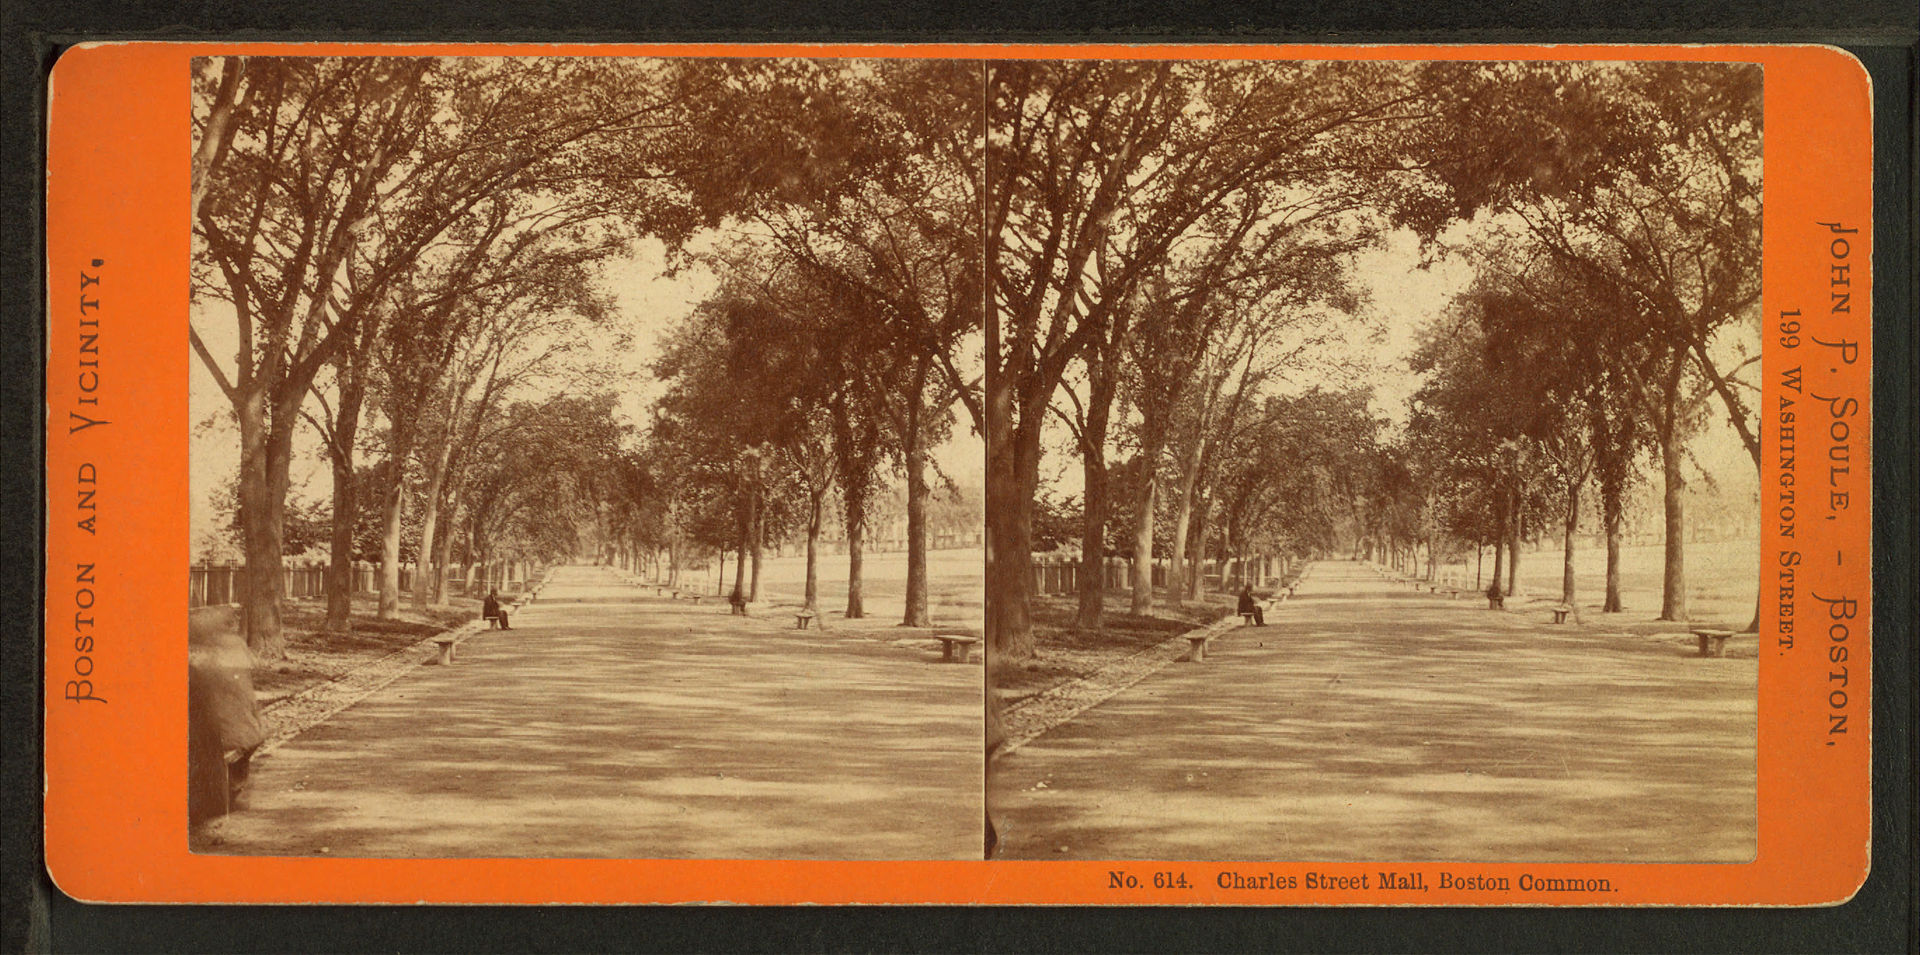
\includegraphics[height= 6cm, width=9cm]{project/images/stereo}
  \caption{\textsc{Stereoscopic Image}}
\end{figure}

 % adds the introduction page
\chapter{History}
\large{\paragraph{}In \emph{280 A.D., Euclid} was the first to recognize that depth perception is obtained when each eye simultaneously receives one of two dissimilar images of the same object. 
	In 1584 \textbf{Leonado da Vinci} studied the perception of depth and, unlike most of contemporaries, produced paintings and sketches that showed a clear understanding of shading, texture and viewpoint projection.Around the year 1600, \textbf{Giovanni Battista della Porta} produced the first artificial 3-D drawing based on Euclid’s notions on how 3-D perception by humans works.}
\large{\paragraph{}
\textbf{Queen Victoria} visited the World's Fair in London in 1851 and was so entranced by the stereoscopes on display that she precipitated an enthusiasm for three-dimensional photography that soon made it a popular form of entertainment world-wide.}
\large{\paragraph{}It was \textbf{Sir Charles Wheatstone} who in 1833 first came up with the idea of presenting slightly different images to the two eyes using a device he called a reflecting mirror stereoscope. When viewed stereoscopically, he showed that the two images are combined in the brain to produce 3-D depth perception. The invention of the Brewster Stereoscope by the Scottish scientist \textbf{Sir David Brewster} in 1849 provided a template for all later stereoscopes. This in turn stimulated the mass production of stereo photography which flourished alongside \emph{mono-photography}. Stereo photography peaked around the turn of the century and went out of fashion as movies increased in popularity.} % adds the Literature Survey page
\chapter{Features of an image}
\section{Image and Video}
\paragraph{} An image is visual representation of a data. While a video can be defined as a collaboration of images. When a particular \emph{frame} is fixed and captured in different time instances, it merges to create a video.
\section{Pixels}
\paragraph{} Image consists of a matrix of pixels, a tuple which contains values of \textbf{Red, Green and Blue} ranging between $ \textsc{(0-255)} $. The combination of values R,G,B determine the colour of the pixel. When video is considered apart from this three, a fourth variable \emph{time} comes in consideration.
\section{Grayscale and binary}
\paragraph{} To compress an Image, \emph{to reduce the bandwidth}, Image is converted into grayscale, or the form where it loses its R,G,B combination and turns black and white. But the \emph{light intensity} is present there, depending upon the intensity regions can be separated in image. This is not possible in binary, as it is completely hindering the color properties, it is \emph{pure black or white} there is no space for intensity.
\section{Object detection}
\paragraph{} Every object class has its own special features that helps in classifying, having unique color or shape. Using those features the object can be extracted.
\chapter{Working}
\paragraph{} Most human beings use what is known as binocular vision to perceive depth and see the world in 3D. The binocular vision system relies on the fact that we have two eyes, which are approximately 3 in apart. This separation causes each eye to see the world from a slightly different perspective. The brain fuses these two views together. It understands the differences and uses them to calculate distance creating our sense of depth and ability to gauge distance.

\paragraph{} If you've ever used a View-Master or a stereoscopic viewer, you have seen your binocular vision system in action. In a View-Master, each eye is presented with an image. Two cameras photograph the same image from slightly different positions to create these images. Your eyes can then correlate these images automatically because each eye sees only one of the images.

\paragraph{} Special kind of Stereo cameras or stereo lenses can be used, which helps in implementing the vision more precisely.

\begin{figure}[!h]
	\begin{subfigure}[b]{0.4\textwidth}
		\centering
		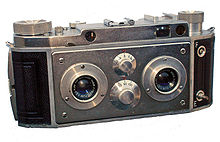
\includegraphics[width=\textwidth]{project/images/Verascope_40.jpg}
		\caption{\textsc{Verascope 40}}
		\label{fig:1}
	\end{subfigure}
	\hspace{3cm}
	\begin{subfigure}[b]{0.4\textwidth}
		\centering
		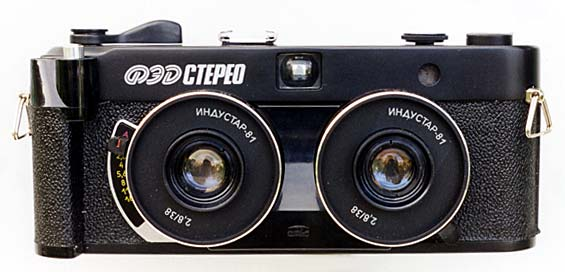
\includegraphics[width=\textwidth]{project/images/fedstereo.jpg}
		\caption{\textsc{FedStereo}}
		\label{fig:2}
	\end{subfigure}
	\caption{\textsc{Stereo Cameras}}
\end{figure}




\chapter{Ways to View Stereoscopic Images}

\paragraph{} There are many ways to view Stereoscopic Images -
%\begin{enumerate}
%	\item Stereo Pairs (stereoscope: separate display for each eye)
%	\item Shutter glasses (most common method)
%	\item Color filter glasses (used in some old 3D movies)
%	\item Polarizing glasses (used in some modern 3D movies)
%\end{enumerate}
\section{Stereo Pairs}
\paragraph{} Typical stereo pair images are two separate images of the same object taken a few inches apart. In this method, the two images are not interlaced but rather presented side by side (left eye image on left and right eye image on right). The images are directly viewable using parallel "free-viewing" glasses which allow each eye to only see its corresponding image.

\section{LCD Shutter Glass Method}
\paragraph{} In the LCD shutter glass 3D display, the left and right images are alternated rapidly on the monitor screen. When the viewer looks at the screen through shuttering eyewear, each shutter is synchronized to occlude the unwanted image and transmit the wanted image. Thus each eye sees only its appropriate perspective view. The left eye sees only the left view, and the right eye only the right view.

\section{Color Filter Glasses}
\paragraph{} Color filter glasses are one of the oldest methods of viewing 3D images or movies. The system works by feeding different images into your eyes. The different color filters allow only one of the images to enter each eye, and your brain does the rest. There are two color filter systems: Red/Blue and Red/Green.

\section{Polarizing Glasses}
\paragraph{} This method is more commonly used in today's 3D movie projections. The audience must wear special glasses which have two polarizing lenses which have their polarization directions adjusted to be 90 degrees different. This makes is possible that left eye sees it's picture without problems but everything ment to right eye (sent out at different polarization) seems to be black. Same applies also to right eye.\\\\

\begin{figure}[H]
	\centering
	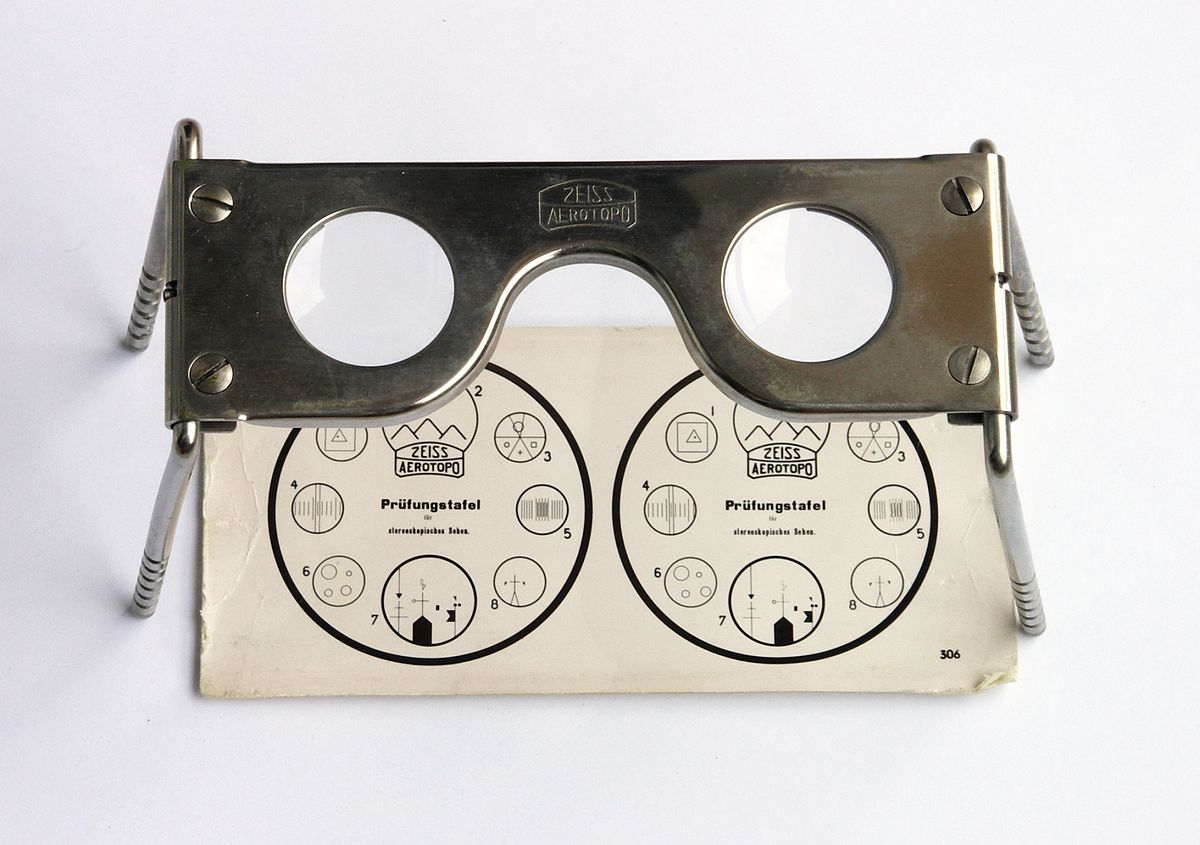
\includegraphics[height= 8cm, width=10cm]{project/images/st.jpg}
	\caption{\textsc{Stereo Glass module}}
\end{figure}

\begin{figure}[H]
	\centering
	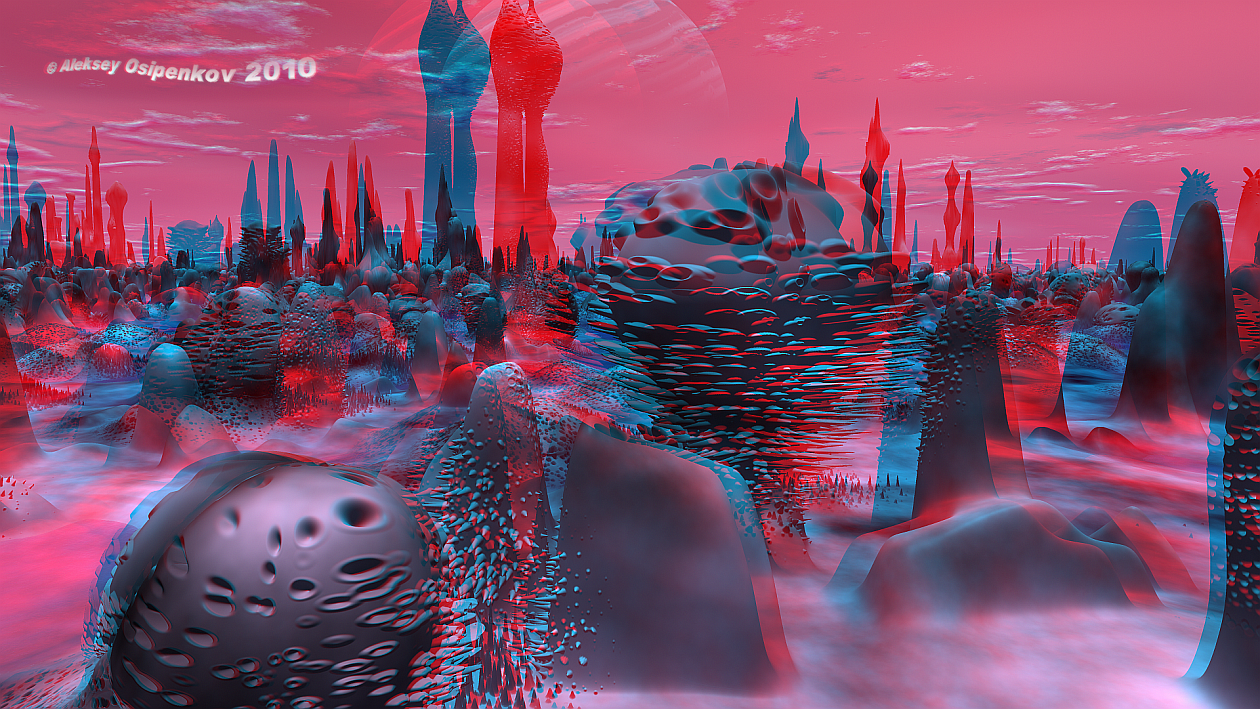
\includegraphics[height= 8cm, width=10cm]{project/images/de.png}
	\caption{\textsc{Image with 3D perception}}
\end{figure}
\chapter{Implementation}
\paragraph{} Stereoscopy is a technique used for recording and representing stereoscopic (3D) images. It can create an illusion of depth using two pictures taken at slightly different positions.
\paragraph{} Stereoscopic picture can be taken with a pair of cameras similarly to our own eyes. The most important restrictions in taking a pair of stereoscopic pictures are the following:
\begin{itemize}
	\item cameras should be horizontally aligned (see Figure 1), and
	\item the pictures should be taken at the same instant.
\end{itemize}

\begin{figure}[!h]
	\begin{subfigure}[b]{0.4\textwidth}
		\centering
		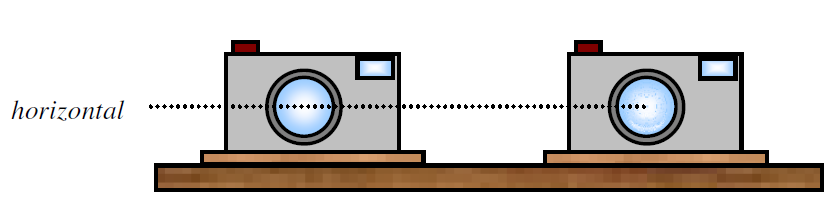
\includegraphics[width=1.3\textwidth,scale=2]{project/images/a.png}
		\caption{\textsc{Horizantal Setup}}
		\label{fig:3}
	\end{subfigure}
	\hspace{2cm}
	\begin{subfigure}[b]{0.4\textwidth}
		\centering
		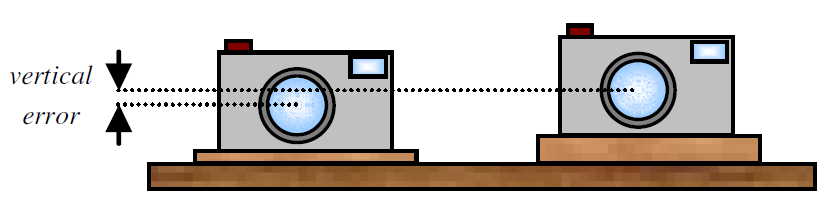
\includegraphics[width=1.3\textwidth]{project/images/b.png}
		\caption{\textsc{Vertical Setup}}
		\label{fig:4}
	\end{subfigure}\\
	\hspace{3cm}
\begin{subfigure}[b]{0.4\textwidth}
	\vspace{1cm}
	
	\centering
	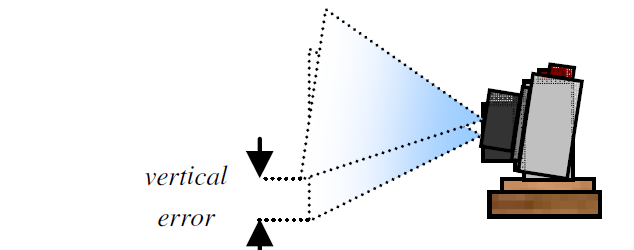
\includegraphics[width=1.3\textwidth]{project/images/c.png}
	\caption{\textsc{Angle Setup}}
	\label{fig:5}
\end{subfigure}
	\caption{\textsc{Stereo Camera Setup}}
\end{figure}
\paragraph{} Stereoscopic pictures allow us to calculate the distance between the camera(s) and the chosen object within the picture. Let the right picture be taken in location SR and the left picture in location SL. B represents the distance between the cameras and is camera’s horizontal angle of view. Object’s position (distance D) can be calculated by doing some geometrical derivations.
We can express distance B as a sum of distances $ B_{1} $ and $ B_{2} $:
\begin{equation}
B=B_{1}+B_{2}= D\tan\varphi_{1}+D\tan\varphi_{2}
\end{equation}
\paragraph{} if optical axes of the cameras are parallel, where $\varphi_{1}$ and $\varphi_{2}$ are angles between optical axis of camera lens and the
chosen object.
Distance D is as follows:
\begin{equation}
D=\frac{B}{\tan\varphi_{1}+\tan\varphi_{2}}
\end{equation}
\begin{figure}[H]
	\centering
	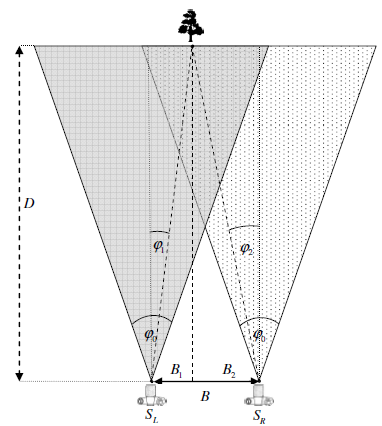
\includegraphics[height= 12cm, width=10cm]{project/images/d.png}
	\caption{\textsc{Object captured by Stereo Setup}}
\end{figure}
This figure shows the setup installed to capture Image of a \emph{tree}, the two cameras used($S_{L}$ and $S_{R}$) are similar in aspect of their \textbf{Field of View}, \textbf{Focal length}.
\newpage
\begin{figure}[h]
	\begin{subfigure}[b]{0.4\textwidth}
		\centering
		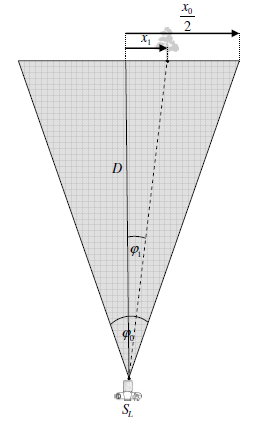
\includegraphics[width=1.3\textwidth,scale=2]{project/images/l.png}
		\caption{\textsc{Object through Left Camera}}
		\label{fig:3}
	\end{subfigure}
	\hspace{2cm}
	\begin{subfigure}[b]{0.4\textwidth}
		\centering
		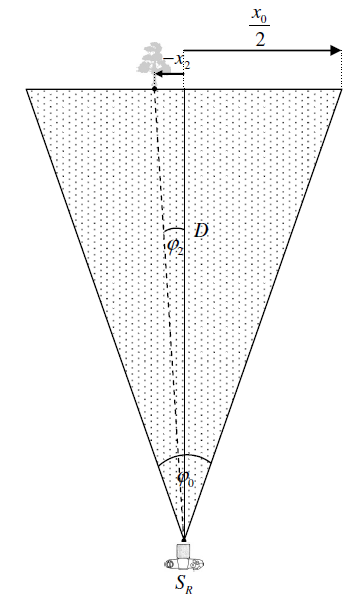
\includegraphics[width=1.3\textwidth]{project/images/r.png}
		\caption{\textsc{Object through Right Camera}}
		\label{fig:4}
	\end{subfigure}\\
	\caption{\textsc{Individual camera working}}
\end{figure}
The two separate images, give rise to two different equations as follows:
\begin{equation}
\frac{x_{1}}{\frac{x_{0}}{2}}=\frac{\tan\varphi_{1}}{\tan\frac{\varphi_{0}}{2}}
\end{equation}
\begin{equation}
\frac{-x_{2}}{\frac{x_{0}}{2}}=\frac{\tan\varphi_{2}}{\tan\frac{\varphi_{0}}{2}}
\end{equation}
Putting the deduced values of $\varphi_{1}$ and $\varphi_{2}$ in the principle equation gives an resultant form of:
\begin{equation}
D=\frac{Bx_{0}}{2\tan(\frac{\varphi_{0}}{2})(x_{1}+x_{2})}
\end{equation}
\textbf{Note:} Here $(x_{1}+x_{2})$ is represented in the form of $(x_{L}-x_{D})$ for ease of understanding.
\newpage
Therefore, if the distance between the cameras (B), number of horizontal pixels $(x_{0})$, the viewing angle of the camera$(\varphi_{0})$ and the horizontal difference between the same object on both pictures $(x_{L}-x_{D})$ are known, then the distance to the object $(D)$ can be calculated as given in  final expression.
The accuracy of the calculated position (distance D) depends on several variables. Location of the object in the right picture can be found within accuracy of one pixel. Each pixel corresponds to the following angle of view:\\
\begin{equation}
\delta=\frac{\varphi_{0}}{x_{0}}
\end{equation}
\\one pixel angle of view $\delta\varphi$ results in distance error $\delta D$. In image we find:
\begin{equation}
\frac{\tan\varphi}{\tan(\varphi-\delta\varphi)}=\frac{\delta D+D}{D}
\end{equation}
Using basic trigonometry identities, the distance error can be expressed as follows:\\
\begin{equation}
\delta D= \frac{D^{2}}{B}\tan(\delta\varphi)
\end{equation}
\begin{figure}[H]
	\centering
	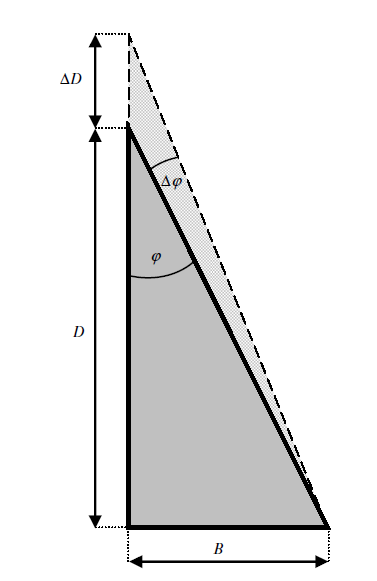
\includegraphics[height= 12cm, width=10cm]{project/images/z.png}
	\caption{\textsc{Distance Error caused by $1$ pixel}}
\end{figure}
\chapter{Object Recognition}
\paragraph{} When the certain object is selected on the left picture, the same object on the right picture has to be automatically located. Let the square matrix $I_{L}$ represent selected object on the left picture. Knowing the properties of stereoscopic pictures (the objects are horizontally shifted), we can define search area within the right picture – matrix $I_{R}$.
Vertical dimensions of $I_{R}$ and $I_{L}$ should be the same, while horizontal dimension of $I_{R}$ should be higher.

\paragraph{}Our next step is to find the location within the search area IR, where the picture best fits matrix $I_{L}$. We do that by subtracting matrix $I_{L}$ from all possible submatrixes (in size of matrix $I_{L}$) within the matrix $I_{R}$. When size of the matrix IL is NxN and size of the matrix $I_{R}$ is $MxN$, where $M>N$, $M-N+1$ submatrixes have to be checked.

\begin{figure}[H]
	\centering
	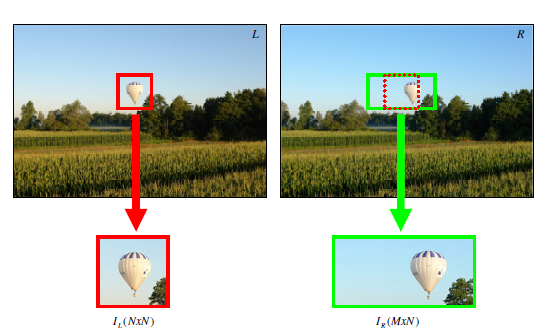
\includegraphics[height= 8cm, width= 14cm]{project/images/y.png}
	\caption{\textsc{Selected object on left picture and search area on right picture.}}
\end{figure}
\paragraph{}The result of each subtraction is another matrix Ii which tells us how similar subtracted images are. More similar two subtracted images are, lower is the mean absolute value of matrix $I_{i}$.\\
\paragraph{} Images in the first example do not match, while in the second example images match almost perfectly.

\paragraph{} The matrix $I_{K}$ with the lowest mean of its elements, represents the location where matrix $I_{L}$ best fits to matrix $I_{R}$. This is also the location of the chosen object within the right image. Knowing the location of the object in the left and right image allow us to calculate the distance between the pictures:\\

\begin{equation}
x_{L}-x_{D}=\frac{N}{2}+K-1-\frac{M}{2}
\end{equation}\\

The distance $(x_{L}-x_{D})$ is the most vital and a bit complex in calculation. This value determines the amount of match between frames captured from both cameras.
Rest of the values are pre-defined and constant, the only value varying is $(x_{L}-x_{D})$. Our work is in finding this value and in turn calculating value of D, which gives the depth.

\chapter{Tools and Libraries}
\paragraph{} \textbf{OpenCV} is an open-source library for computer vision. It is used for capturing image, and extract features from it which ultimately leads to feature extraction and object detection.
\paragraph{} \emph{Grayscale and thresholding} of image is also done using OpenCV. Also capping by colour, Canny edge detection, erosion and dilation, contour search, and moments (to find centre of frame) are implemented using CV.


\begin{figure}[H]
  \centering
    
\includegraphics[scale=0.4]{project/images/cv}
  \caption{\textbf{OpenCV}}
\end{figure}

\paragraph{} Python language is used along with numpy distribution for numerical computation. Also Scipy is used for final distance/depth calculation.

\begin{figure}[H]
	\centering
	
\includegraphics[scale=0.4]{project/images/py}
	\caption{\textbf{Numpy \& Python}}
\end{figure}


 % adds the Project Design
\chapter{Algorithm \& Code}
\section{Importing modules}
\begin{lstlisting}
from scipy.spatial import distance as dist
import numpy as np
import cv2
\end{lstlisting}
This are the distributions to be used.

\section{Capture and Work on image}
\begin{lstlisting}
cap0=cv2.VideoCapture(0)
while(1):
	ret,img1=cap0.read()
	image_blur = cv2.GaussianBlur(img1, (7, 7), 0)
	image_blur_hsv1 = cv2.cvtColor(image_blur, cv2.COLOR_BGR2RGB)
\end{lstlisting}
In this section, OpenCV is capturing live feed from HDcam, and the individuals frames are extracted, Gaussian Blur filter is applied and the image format is changed from BGR to HSV.

\section{Colour grading}
\begin{lstlisting}
max_orange = np.array([245,136,99])
min_orange = np.array([150,45,10])
max_white= np.array([225,224,228])
min_white=np.array([119,115,136])
mask1 = cv2.inRange(image_blur_hsv1,min_orange,max_orange)
mask2 = cv2.inRange(image_blur_hsv1,min_white,max_white)
mask=mask1+mask2
\end{lstlisting}
In this section, OpenCV is thresholding orange an white color, with some predefined values of R,G,B combination. The mask is created and applied on the blurred image.

\section{Canny edge and Contour}
\begin{lstlisting}
edged1 = cv2.Canny(mask, 50, 100)
edged1 = cv2.dilate(edged1, None, iterations=1)
edged1 = cv2.erode(edged1, None, iterations=1)

 _,contours1,_ = cv2.findContours(edged1, cv2.RETR_TREE,cv2.CHAIN_APPROX_SIMPLE)
\end{lstlisting}
Here, Canny edge detection done and image dilated and eroded for finding features and then contours are scratched out by edges.

\section{Finding co-ordinates}
\begin{lstlisting}
M1=cv2.moments(contours1)
if M1["m00"] != 0:
	cX1=int(M1['m10']/M1["m00"])
	cY1=int(M1["m01"]/M1["m00"])
	cv2.drawContours(img1,c1, -1, (0, 255, 0), 2)
	cv2.circle(img1, (cX1, cY1), 7, (255, 255, 255), -1)
	cv2.putText(img1, "center", (cX1 - 20, cY1 - 20),cv2.FONT_HERSHEY_SIMPLEX, 0.5, (255, 255, 255), 2)
else:
	cX1,cY1=0,0
	c2 = max(contours2, key = cv2.contourArea)
\end{lstlisting}
Here the co-ordinate of the detected image is obtained, and the distance of object from the center of frame is determined.

\section{Finding co-ordinates}
\begin{lstlisting}
 D=cX1+cX2
\end{lstlisting}
Finally the depth is calculated as sum of $C_{x1}$ and $C_{x2}$ which are the distance returning $x_{L}-x_{D}$.




\chapter{Conclusion and Future Scope}
\section{Conclusion}
\paragraph{}This distance
measurement is based upon the pictures taken from two
horizontally displaced cameras. The user should select the
object on left camera and the algorithm finds similar object
on the right camera. From displacement of the same object
on both pictures, the distance to the object can be calculated.
Although the method is based on relatively simple
algorithm, the calculated distance is still quite accurate.
Better results are obtained with wider base (distance between
the cameras). This is all according to theoretical derivations.
\begin{itemize}
	\item Visible light is used as mode of communication, hence no hustle of Radio Frequencies.
	\item This is an accurate way of calculating depth of object in passive manner.
	\item It has wide range of application, from medical science to research.
	\item Now a days, it is implemented in Smartphone cameras to improvise autofocus.
	
\end{itemize}
\newpage
\section{Future Scope}
\paragraph{}Recent advances in 3-dimensional (3-D) stereoscopic imaging have enabled 3-D display technologies in the operating room. We find 2 beneficial applications for the inclusion of 3-D imaging in clinical practice. The first is the real-time 3-D display in the surgical theater, which is useful for the neurosurgeon and observers. In surgery, a 3-D display can include a cutting-edge mixed-mode graphic overlay for image-guided surgery. The second application is to improve the training of residents and observers in neurosurgical techniques. This article documents the requirements of both applications for a 3-D system in the operating room and for clinical neurosurgical training, followed by a discussion of the strengths and weaknesses of the current and emerging 3-D display technologies. An important comparison between a new autostereoscopic display without glasses and current stereo display with glasses improves our understanding of the best applications for 3-D in neurosurgery. Today's multiview autostereoscopic display has 3 major benefits: It does not require glasses for viewing; it allows multiple views; and it improves the workflow for image-guided surgery registration and overlay tasks because of its depth-rendering format and tools. Two current limitations of the autostereoscopic display are that resolution is reduced and depth can be perceived as too shallow in some cases. Higher-resolution displays will be available soon, and the algorithms for depth inference from stereo can be improved. The stereoscopic and autostereoscopic systems from microscope cameras to displays were compared by the use of recorded and live content from surgery. To the best of our knowledge, this is the first report of application of autostereoscopy in neurosurgery. % adds the Scheduling and Planning page
\addcontentsline{toc}{chapter}{References}
\begin{thebibliography}{99}

\end{thebibliography}

[1] M. Vidmar, ABC sodobne stereofotografije z maloslikovnimi
kamerami, Cetera, 1998.\\
$[2]$ H. Walcher, Position sensing – Angle and distance
measurement for engineers, Second edition, Butterworth-
Heinemann Ltd., 1994.\\
$[3]$ D. Vrancic and S. L. Smith, Permanent synchronization of
camcorders via LANC protocol, Stereoscopic displays and virtual
reality systems XIII : 16-19 January, 2006, San Jose, California,
USA, (SPIE, vol. 6055).\\
$[4]$ Navigation 2, Radio Navigation, Revised edition, Oxford
Aviation Training, 2004.\\
$[5]$ P. Gedei, Ena in ena je tri, Monitor, july 2006,
http://www.monitor.si/clanek/ena-in-ena-je-tri/, (21.12.2007).\\
$[6]$ J. Carnicelli, Stereo vision: measuring object distance using
pixel offset,\\ http://www.alexandria.nu/ai/blog/entry.asp?E=32,
(29.11.2007).\\
$[7]$ A. Klein, Questions and answers about stereoscopy,\\
http://www.stereoscopy.com/faq/index.html, (28.1.2007).\\
$[8]$ A. Woods, Image distortions and stereoscopic video systems,\\
http://www.3d.curtin.edu.au/spie93pa.html, (27.1.2007). % adds the References page

\end{document}